


\input 05-tjz

\vfill
\spis{Odwzorowania addytywne i~geometria}
{Franciszek Hansdorfer}

\wtyt{Odwzorowania addytywne i~geometria}

\waut{Franciszek HANSDORFER}

Rozważmy zbiór \marg{Artykuł jest skrótem pracy z~45. edycji
Konkursu Uczniowskich Prac z~Matematyki im. Pawła Domańskiego. Z~pełną jej
wersją można zapoznać się na stronie \href{http://deltami.edu.pl}{\tt deltami.edu.pl}. Autor chciałby bardzo podziękować dr. hab. Mariuszowi Skałbie za opiekę merytoryczną.}
\[K= \{a+b\sqrt{2} : a,b \in \mathbb Q\}.\]

Do tego zbioru należą zatem liczby $1+2\sqrt{2}$ czy
$\frac{2}{3}+\frac{1}{8}\sqrt{2}$. Oczywiście należą do niego wszystkie liczby
wymierne (wystarczy wziąć $b=0$), w~tym liczby $0$ i~$1$. Ponadto jeśli wezmę dowolne dwie
liczby z~$K$, to ich suma i~różnica również należą do $K$. Tak samo jest
z~iloczynem, o~czym przekonuje nas poniższa równość: \begin{equation*}
(a+b\sqrt{2})\cdot (c+d\sqrt{2})= (ac+2bd) + (bc+ad)\sqrt{2}.
\end{equation*}
\marg{\vspace*{0cm}
Strukturę, której elementy możemy dodawać, odejmować, mnożyć i~dzielić
z~wyróżnionymi elementami 0 (którego dodanie nic nie zmienia) i~1 (mnożenie przez które nic nie
zmienia), nazywamy \textit{ciałem}. Ciałem jest zatem zbiór liczb
rzeczywistych, wymiernych, lecz również opisany tu zbiór $K.$
}%
Operacja dzielenia też nie wyprowadza poza $K$, w~czego uzasadnieniu pomaga szkolna sztuczka na
pozbywanie się niewymierności z~mianownika:
\begin{equation*}
\frac{a+b\sqrt{2}}{c+d\sqrt{2}}= 
\frac{(a+b\sqrt{2})(c-d\sqrt{2})}{(c+d\sqrt{2})(c-d\sqrt{2})}= 
\frac{ac-2bd}{c^2-2d^2} + \frac{bc-ad}{c^2-2d^2}\sqrt{2}.
\end{equation*}

Zdefiniujmy teraz funkcję $\sigma: K\to K$ wzorem:
\[\sigma(a+b\sqrt{2}) = a-b\sqrt{2}.\]
\marg{Dla $x\in K$ liczbę $\sigma(x)$ nazywa się często
\textit{sprzężeniem}~$x$.}%
Przekształcenie $\sigma$ w~ten sposób zdefiniowane ma ciekawe własności.
Zacznijmy od tego, że dobrze się ono zachowuje ze względu na dodawanie
i~mnożenie. 
Niech $x=a+b\sqrt{2}$, $y=c+d\sqrt{2}$, gdzie $a,b,c,d\in\mathbb{Q}$. Wtedy:
\begin{equation*}
\begin{split}
\sigma(x+y)&=\sigma(a+c+(b+d)\sqrt{2})=a+c-(b+d)\sqrt{2}\\&=a-b\sqrt{2}
+c-d\sqrt{2}=\sigma{(x)}+\sigma{(y)},\\
\sigma(xy) & =\sigma\left((a+b\sqrt{2})(c+d\sqrt{2})\right)=\sigma(ac+ad\sqrt{2}+bc\sqrt{2} +2bd ) \\& = \sigma\left((ac+2bd)+(ad+bc)\sqrt{2}\right)=(ac+2bd)-(ad+bc)\sqrt{2}\\  & = (a-b\sqrt{2})(c-d\sqrt{2}) = \sigma(x)\sigma(y).
\end{split}
\end{equation*}
Pokazaliśmy, że $\sigma$ jest \textit{addytywna}
i~\marg{\vspace*{0cm}Przedstawione tu własności pozwalają nazwać funkcję
$\sigma$ \textit{automorfizmem} ciała~$K.$}
\textit{multiplikatywna}. Co istotne, zachowuje ona elementy neutralne  dodawania
i~mnożenia, czyli 0 i~1 -- rzeczywiście, $\sigma(0)=0$ oraz $\sigma(1)=1$.

Chociaż $\sigma$ jest bardzo \emph{porządną} funkcją z~algebraicznego punktu
widzenia, to z~analitycznego punktu widzenia już taka regularna nie jest.
Wykażemy mianowicie, że $\sigma$ nie jest
ciągła w~żadnym punkcie.
Przypomnijmy najpierw definicję  Heinego ciągłości funkcji:
\begin{gather*}
\mbox{\emph{$f$ jest ciągła w~punkcie $x_0$ wtedy i~tylko wtedy, gdy:}}
\\
\forall{(x_n)}:\lim_{n\to\infty} x_n =x_0 \implies \lim_{n\to\infty} f(x_n)=f(x_0).
\end{gather*}
Niech więc $x_0 = a+b\sqrt{2}$, gdzie $a,b\in \mathbb Q$.

Definiujemy teraz ciąg $x_n = a+b\sqrt{2}+{(1-\sqrt{2})}^n$. Ponieważ
$|1-\sqrt{2}|<1$, więc
\[\lim_{n\to\infty} x_n = a+b\sqrt{2} = x_0.\]

Korzystając z~własności funkcji $\sigma$, mamy:
\[\sigma(x_n) = \sigma\big(a+b\sqrt{2}+(1-\sqrt{2})^n\big) = a-b\sqrt{2} + (1+\sqrt{2})^n.\vadjust{\eject}\]
Ponieważ $1+\sqrt{2}>1$, więc ciąg $(\sigma(x_n))$ jest rozbieżny. Zatem:
%\[\lim_{n\to\infty} \sigma (x_n) \neq \sigma (x_0).\]
\[ \sigma (x_n) \not\to \sigma (x_0).\]
\marg{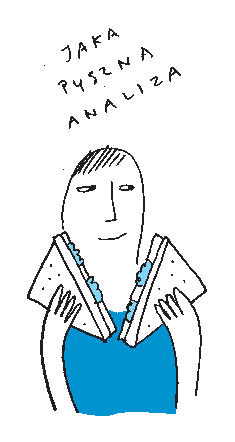
\includegraphics{art/202501_kol12}}Dowiedliśmy więc, że $\sigma$ jest nieciągła w dowolnie
wybranym punkcie $x_0 \in K$.

Spróbujemy teraz zbadać funkcję $\sigma$ pod względem geometrycznym. W~tym celu potrzebujemy odpowiednika funkcji $\sigma$ zdefiniowanego na ,,płaszczyźnie''. Niech więc $F:K^2 \to K^2$ będzie dla $x,y \in K$ określone wzorem:
\[F(x,y) = (\sigma(x), \sigma(y)).\]
Tak zdefiniowane $F$ ma bardzo ciekawe, paradoksalne wręcz, własności.
Z jednej strony $F$ jest bardzo nieregularne, bo wszędzie nieciągłe, co wynika z~wyżej udowodnionej nieciągłości $\sigma$.

Z drugiej jednak strony $F$ jest bardzo regularne, gdyż jest addytywne. Otóż dla $x_1,y_1,x_2,y_2 \in K$ mamy:
\begin{align*}
    F((x_1,y_1) + (x_2,y_2)) & = F(x_1+x_2, y_1+y_2) = (\sigma(x_1+x_2), \sigma(y_1+y_2)) \\&= (\sigma(x_1)+\sigma(x_2), \sigma(y_1)+\sigma(y_2)) = F(x_1,y_1) + F(x_2,y_2).
\end{align*}
Analogicznie możemy uzasadnić, że dla dowolnych $\alpha,x_1,x_2\in K$
zachodzi $F(\alpha\cdot(x_1,x_2))=\sigma(\alpha)\cdot F(x_1,x_2)$.

Co dla nas najważniejsze, z~geometrycznego punktu widzenia $F$
zachowuje pewne podstawowe własności geometryczne.
Po pierwsze, $F$ zachowuje współliniowość punktów. Wynika to
z~faktu, że jeśli $X=(x_1,x_2)$, $Y=(y_1,y_2)$ i~$Z=(z_1,z_2)$ są współliniowymi
punktami z~$K^2$, to $X-Y=\alpha\cdot(X-Z)$ dla pewnej liczby $\alpha\in K$, a~stąd
$F(X)-F(Y)=\sigma(\alpha)\cdot\big(F(X)-F(Z)\big)$. Dlatego obrazami prostych
(w~obcięciu do $K^2$) w~przekształceniu $F$ są proste. Ponieważ jednak funkcja $\sigma$
może zmienić znak lub zamienić liczbę o~module większym od 1 na taką o~module
mniejszym od 1 (np. dla $\alpha=1+\sqrt{2}$), obrazami odcinków nie są odcinki.

Ponadto $F$ zachowuje \textbf{równość odległości}, czyli dla $X,Y,Z,T \in K^2$ mamy:
\begin{equation}
    d(X, Y) = d(Z, T) \implies d(F(X), F(Y)) = d(F(Z), F(T)),
\end{equation}
gdzie przez $d(\cdot ,\cdot)$ oznaczamy euklidesową odległość na
płaszczyźnie.
\marg{\vspace*{-1cm}    {\hspace*{-1.2cm}\begin{tikzpicture}
        \begin{axis}[
                width = 1.2\linewidth,
                height = 1.2\linewidth,
                axis lines=middle,
                ymajorgrids=true,
                xmajorgrids=true,
                xmin=-1.5,
                xmax=5.4,
                ymin=-1.5,
                ymax=5.4,
                xtick={-1,0,...,5},
                ytick={-1,0,...,5},]
            \begin{scriptsize}
                \filldraw[magenta, thick] (1,2.41421) -- (3.41421, 3.41421);
                \filldraw[magenta, thick] (-1,2.41421) -- (0,4.82843);
                \filldraw[black] (1,2.41421) circle (1pt) node[anchor=north east]{$P_1$};
                \filldraw[black] (3.41421, 3.41421) circle (1pt) node[anchor=south west]{$P_2$};
                \filldraw[black] (-1,2.41421) circle (1pt) node[anchor=north]{$Q_1$};
                \filldraw[black] (0,4.82843) circle (1pt) node[anchor=west]{$Q_2$};
                \filldraw[red, thick] (1, -0.414214) -- (0.585786, 0.585786);
                \filldraw[red, thick] (0, 0.585786) -- (1, 0.171573);
                \filldraw[black] (1, -0.4142141) circle (1pt) node[anchor=north]{$F(P_1)$};
                \filldraw[black] (0.585786, 0.585786) circle (1pt) node[anchor=south]{$F(P_2)$};
                \filldraw[black] (0, 0.585786) circle (1pt) node[anchor= east]{$F(Q_1)$};
                \filldraw[black] (1, 0.171573) circle (1pt) node[anchor= west]{$F(Q_2)$};
            \end{scriptsize}
        \end{axis}
    \end{tikzpicture}}\\[4pt]
		Rys. 1 
    }
Sprawdzenie jest proste. Niech $X = (x_1, x_2), Y= (y_1, y_2), Z=(z_1,z_2), T=(t_1,t_2)$. Ponieważ
$d((x_1,x_2), (y_1, y_2)) = d((z_1, z_2), (t_1, t_2))$, więc
\[(y_1-x_1)^2 + (y_2-x_2)^2 =(t_1-z_1)^2 + (t_2 - z_2)^2.\]
Do obu stron przykładamy funkcję $\sigma$:
\[(\sigma(y_1) -\sigma(x_1))^2 +(\sigma(y_2) - \sigma(x_2))^2 = (\sigma(t_1) - \sigma(z_1))^2 + (\sigma(t_2) - \sigma(z_2))^2 .\]
Zatem
\[d(F(X), F(Y)) = d(F(Z), F(T)).\]

To, że $F$ zachowuje równość odległości, nie oznacza jednak, że jest izometrią.
Na przykład dla punktów $P_1 = (1,1+\sqrt{2}), P_2 = (2 + \sqrt{2}, 2 +
\sqrt{2}),$ ${Q_1 = (-1,1+\sqrt{2}), Q_2 = (0,2+2\sqrt{2})}$ mamy
$d(P_1,P_2) = d(Q_1, Q_2)$. Ale na mocy~(1) mamy też $d(F(P_1), F(P_2)) =
d(F(Q_1), F(Q_2))$, jednakże, jak można zobaczyć na rysunku 1 (lub obliczyć),
$d(P_1,P_2) \neq d(F(P_1), F(P_2))$.

\marg{\vspace*{-.8cm}
\hspace*{-.8cm}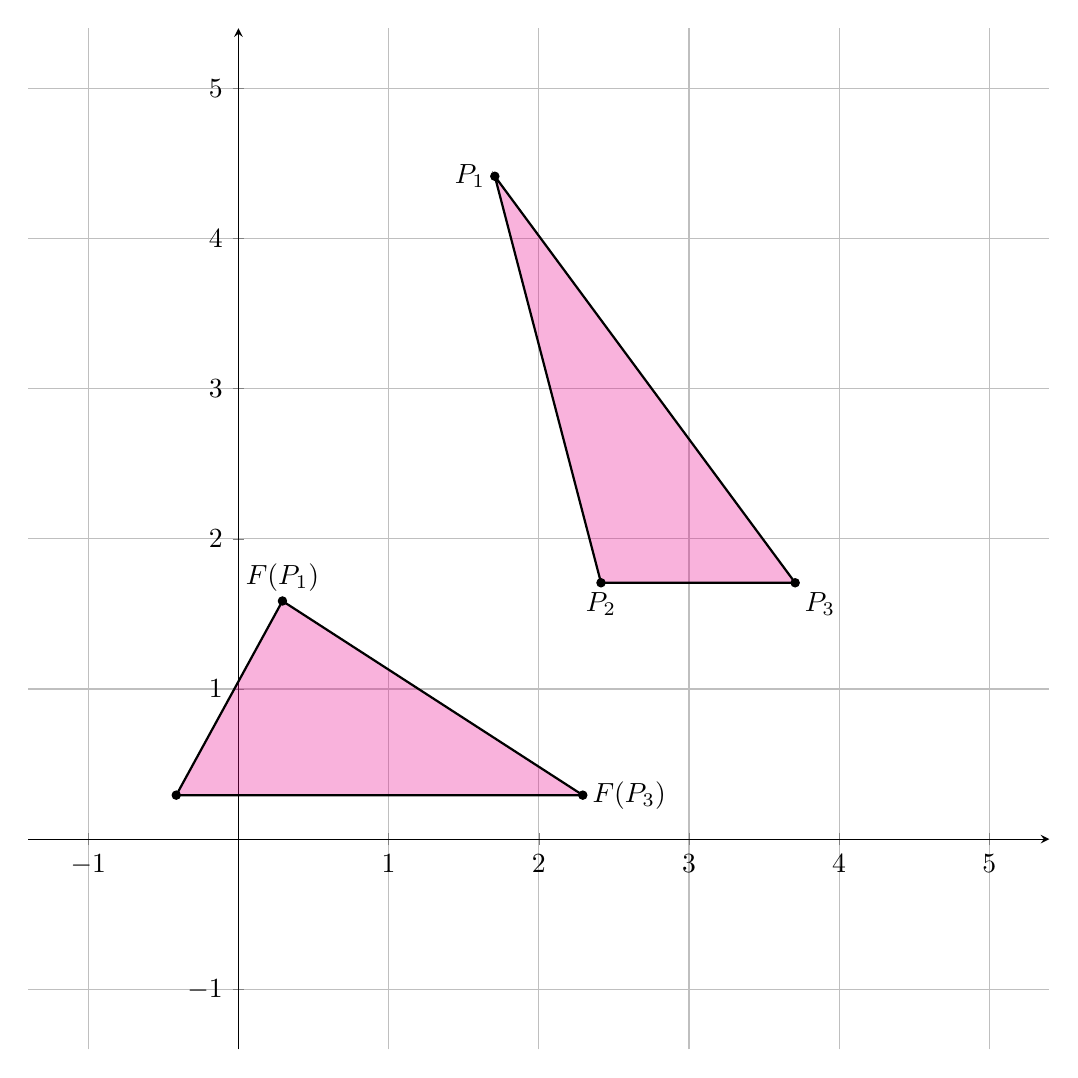
\begin{tikzpicture}%[scale=.85]
        \begin{axis}[
                width = 1.2\linewidth,
                height = 1.2\linewidth,
                axis lines=middle,
                ymajorgrids=true,
                xmajorgrids=true,
                xmin=-1.4,
                xmax=5.4,
                ymin=-1.4,
                ymax=5.4,
                xtick={-2,-1,0,...,5},
                ytick={-1,0,...,5},]
            \begin{scriptsize}
                \filldraw[color=black, fill=magenta,fill opacity=0.3, thick] (1.70711, 4.41421) -- (2.41421, 1.70711) --(3.70711, 1.70711)-- cycle;
                \filldraw[black] (1.70711, 4.41421) circle (1.5pt) node[anchor=east]{$P_1$};
                \filldraw[black] (2.41421, 1.70711) circle (1.5pt) node[anchor=north]{$P_2$};
                \filldraw[black] (3.70711, 1.70711) circle (1.5pt) node[anchor=north west]{$P_3$};
                \filldraw[color=black, fill=magenta,fill opacity=0.3, thick] (0.292893, 1.58579) -- (-0.414214, 0.292893) -- (2.29289, 0.292893) -- cycle;
                \filldraw[black] (0.292893, 1.58579) circle (1.5pt) node[anchor=south]{$F(P_1)$};
                \filldraw[black] (-0.414214, 0.292893) circle (1.5pt) node[anchor=east]{};%$F(P_2)$};
                \filldraw[black] (2.29289, 0.292893) circle (1.5pt) node[anchor=west]{$F(P_3)$};
            \end{scriptsize}
        \end{axis}
      \end{tikzpicture}\raise31.5pt\llap{$F(P_{2})$\kern94pt}\\[4pt]
		Rys. 2. Przekształcenie $F$ może zamienić
		wierzchołki trójkąta ostrokątnego na
		rozwartokątnego. Na powyższym rysunku mamy $P_1 = (1+\frac{\sqrt{2}}{2},3+\sqrt{2}),
P_2 = (1+\sqrt{2},1+\frac{\sqrt{2}}{2}), P_3 =
(3+\frac{\sqrt{2}}{2},1+\frac{\sqrt{2}}{2})$
		}
		Poza tym $F$ zachowuje prostopadłość wektorów. Niech $X, Y, Z \in K^2$
		i~załóżmy, że $\angle YXZ=90^\circ$, czyli $\langle X-Y, X-Z\rangle =0$:
\[( x_1-y_1 )( x_1-z_1 ) + ( x_2-y_2 )( x_2-z_2 ) = 0.\]
Po przyłożeniu funkcji $\sigma$ do obu stron otrzymujemy:
\[\big( \sigma(x_1)-\sigma(y_1) \big)\big( \sigma(x_1)-\sigma(z_1) \big) + \big(
\sigma(x_2)-\sigma(y_2) \big)\big( \sigma(x_2)-\sigma(z_2) \big) =
\sigma(0)=0,\]
czyli
\[\angle F(Y)F(X)F(Z) = 90^\circ.\]

		W ogólności przekształcenie $F$ nie zachowuje jednak kątów między
		prostymi, co ilustruje rysunek~2.

Przekształcenie $F$ godzi w~sobie sprzeczne natury: \emph{dziką} naturę
analityczną (nigdzie nie jest ciągłe) i~\emph{łagodną} naturę
algebraiczno-geometryczną (jest addytywne, zachowuje równość odległości
i~prostopadłość wektorów).  Zachęcam Czytelnika do własnych badań nad jego
własnościami!



